\documentclass[10pt,a4paper]{article}
\usepackage[top=3cm,bottom=3cm,includeheadfoot]{geometry}	% Seitengeometrie festlegen
\usepackage[ngerman]{babel}
\usepackage{fancyhdr}						% das nötige Paket um Fuß- / Kopfzeilen zu verwenden			
\usepackage[utf8]{inputenc}
\usepackage{amsmath}
\usepackage{amsfonts}
\usepackage{amssymb}
\usepackage{caption}
\usepackage{listings}
\usepackage{textcomp}
\usepackage{graphicx}
\usepackage{color}
\newcommand{\hilight}[1]{\colorbox{yellow}{#1}}
\usepackage{chngcntr}
\usepackage{hyperref}
\usepackage{caption}

\counterwithin{figure}{section}

\author{Ken Hasenbank, Artur Schmidt}
\title{Praktikum 1}
\date{3.11.2017}

\pagestyle{fancy}	%ermöglicht die Verwendung von eigens bearbeiteten Kopf-/ Fußzeilen
\fancyhf{}
%Bearbeiten der Kopzeile
\fancyhead[R]{\thepage}
\fancyhead[C]{Chaos \& Fraktale}
\fancyhead[L]{3.11.2017}
\renewcommand{\headrulewidth}{0.4pt} %obere Trennlinie
%Bearbeiten der Fußzeile
\fancyfoot[C]{ \centering Ken Hasenbank,\linebreak Artur Schmidt}
\renewcommand{\footrulewidth}{0.4pt} %untere Trennlinie


\begin{document}
%\thispagestyle{empty}		% legt ein für diese Seite ein Layout fest, dass leer ist (keine Fuß-/ Kopfzeile etc) 

%%%%%%%%%%%%  DECKBLATT ANFANG   %%%%%%%%%%%%%%
\begin{titlepage}
\begin{center}
	\Large{Hochschule Darmstadt}\\
	\large{Fachbereich Informatik}
\end{center}

\vspace{1cm}
\begin{center}
	\large{Chaos und Fraktale}
\end{center}

\vspace{2,5cm}
\begin{center}
	\huge{Praktikum}\\
\end{center}

\begin{center}
	\Huge{\textbf{Praktikumsaufgabe 1}} 
\end{center}


\vspace{6cm}
\begin{center}
{\large 
\begin{tabular}{lll}
	Semester: && SoSe 2017\\
	\vspace{1mm}\\
	Laboranten: && Ken Hasenbank\\
	&& Artur Schmidt\\
	\vspace{1 mm}\\
	Datum:	&& 03.11.2017\\
	\end{tabular} 
	}%\large beenden
\end{center}

\end{titlepage}
%%%%%%%%%%%%  DECKBLATT ENDE  %%%%%%%%%%%%%%5

\tableofcontents
\newpage
In diesem Laborversuch soll ein System auf dessen Echtzeiteigenschaften Untersucht werden. Hierzu werden mittels des Messtools von Keil \textmu{}Vision die Ausführungszeiten gemessen und daraufhin überprüft, ob sie kleiner als die obere Schranke von 400 \textmu{}s sind. Als Anwendung dient hierbei die in der Laboraufgabe 1 entwickelte Fahrstuhlsteuerung. 
\section{Einleitung}
In diesem Laborversuch soll ein Nachweise echter Echtzeiteigenschaften erfolgen. Dies ist deshalb so wichtig, weil es bei eingebetteten Systemen nicht ohne weiteres Möglich ist neue Software aufzuspielen und so nachträglich Softwarefehler zu beheben. Weiterhin macht die in der Regel hohe Stückzahl ein nachträgliches Austauschen der 
\newpage
\section{Codeanalyse}

%\begin{center}
%	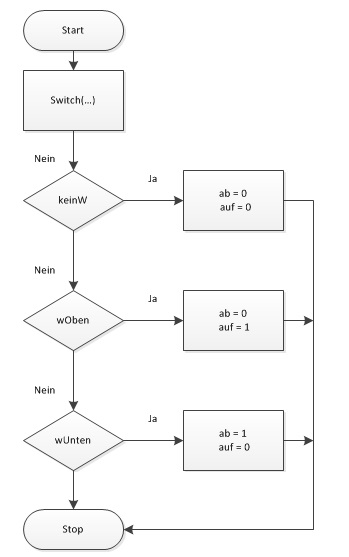
\includegraphics[scale=1]{Screens/switch_case_ausgabefkt.jpg}
%	\captionof{figure}{Ausgabefunktion der Berechnungsphase per switch-case-Anweisung}
%	\label{fig:switchCaseAusgabe}
%\end{center}
\ \\


\newpage
\section{Testfolge}

\ \\
\section{Auswertung}
\section{Anhang}
\subsection{Code}
%HIER KÖNNEN WIR DEN CODE LINKEN!
\lstinputlisting
    [caption={Quellcode}
       \label{lst:cClass},
       captionpos=t,language=C]
 {Screens/main.c}
\subsection{Zustandsautomat}

%\begin{center}
%	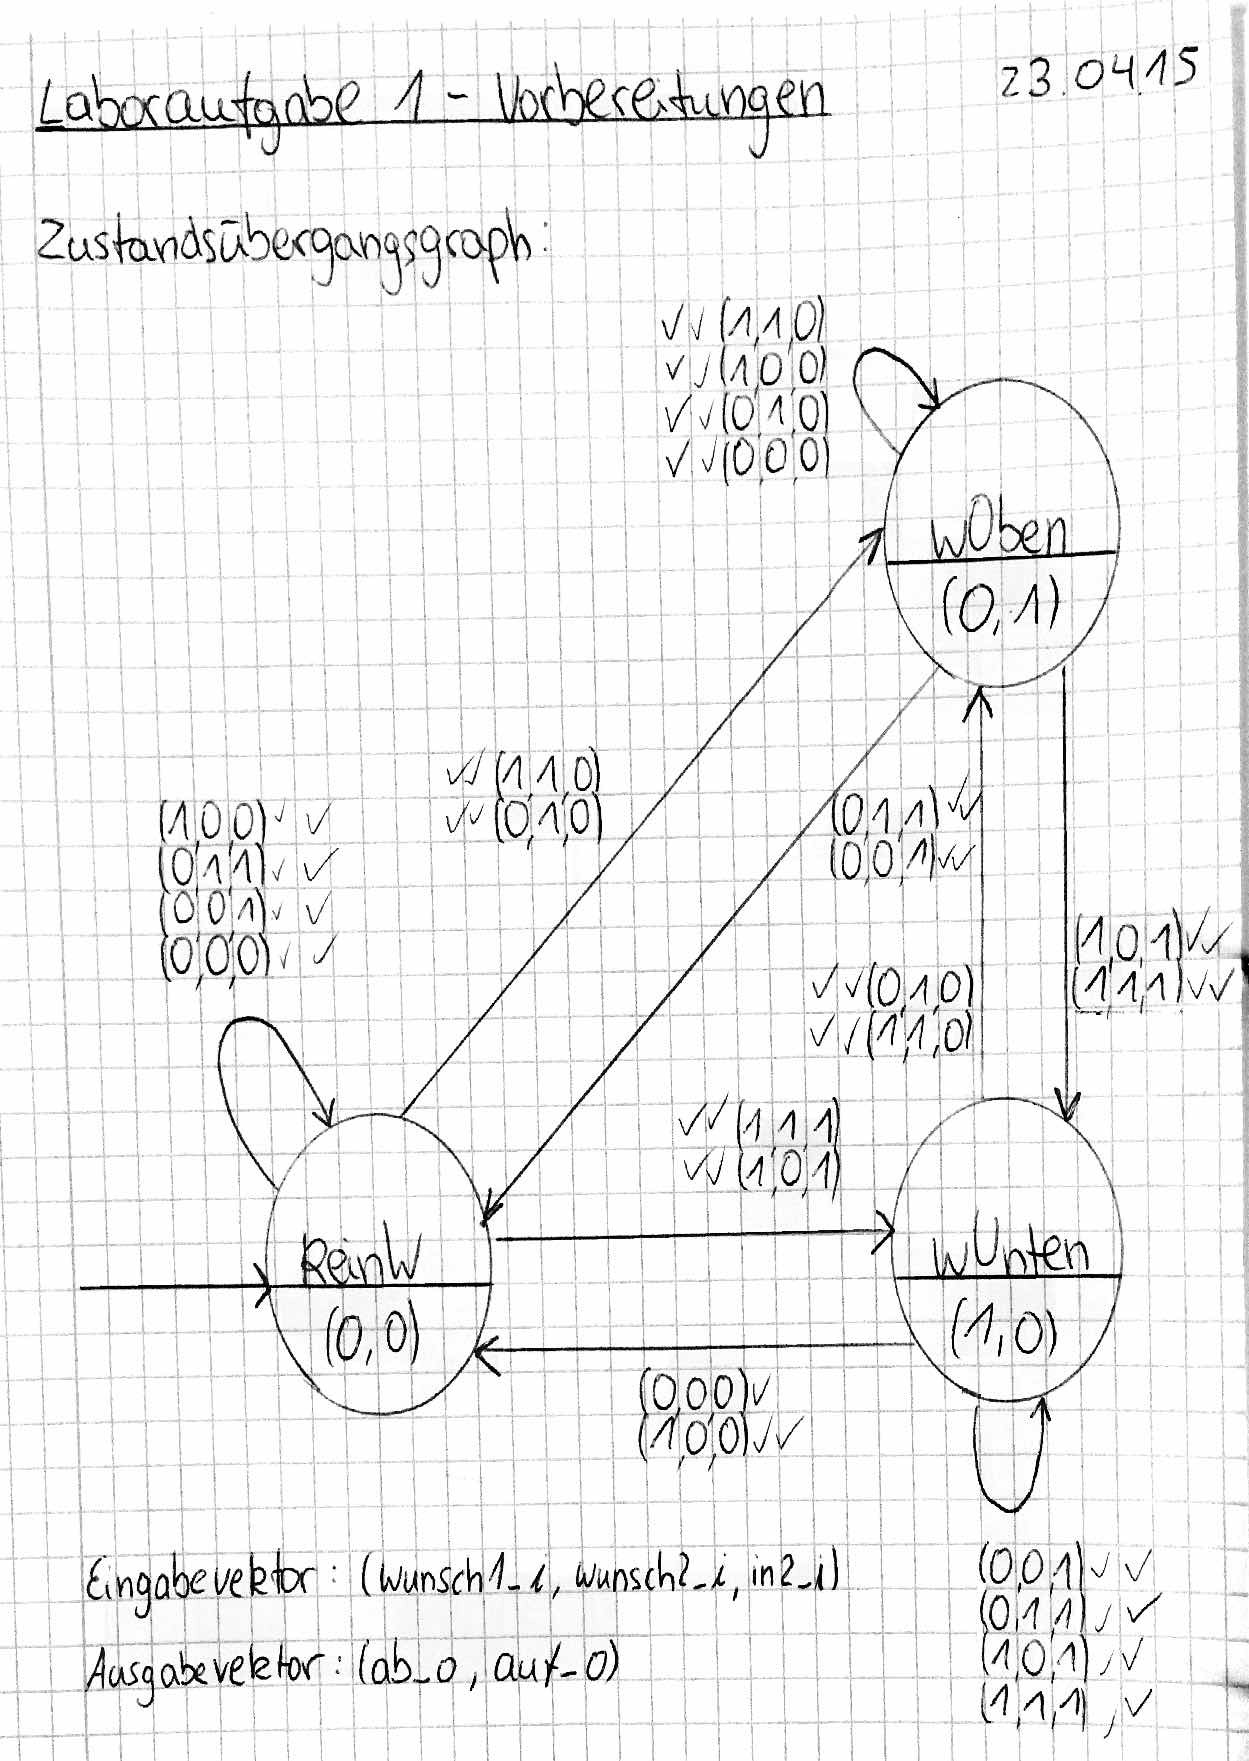
\includegraphics[scale=0.3]{Screens/IMG_4365.jpg}
%	\captionof{figure}{Zustandsautomat der Fahrstuhlsteuerung}
%	\label{fig:automat}
%\end{center}

\subsubsection{Testfolge für die vollständige Zustandsübergangsabdeckung}
\hilight{HIER DIE TABELLE mit dem Label Zustand EINFÜGEN! DANKE!}
\end{document}